\documentclass[border=10pt]{standalone}

\usepackage{tikz}
\usepackage{tikzsymbols}
\usetikzlibrary{calc,patterns,shapes.geometric}

\def\centerarc[#1](#2)(#3:#4:#5){\draw[#1] ($(#2)+({#5*cos(#3)},{#5*sin(#3)})$) arc (#3:#4:#5);}

\begin{document}
	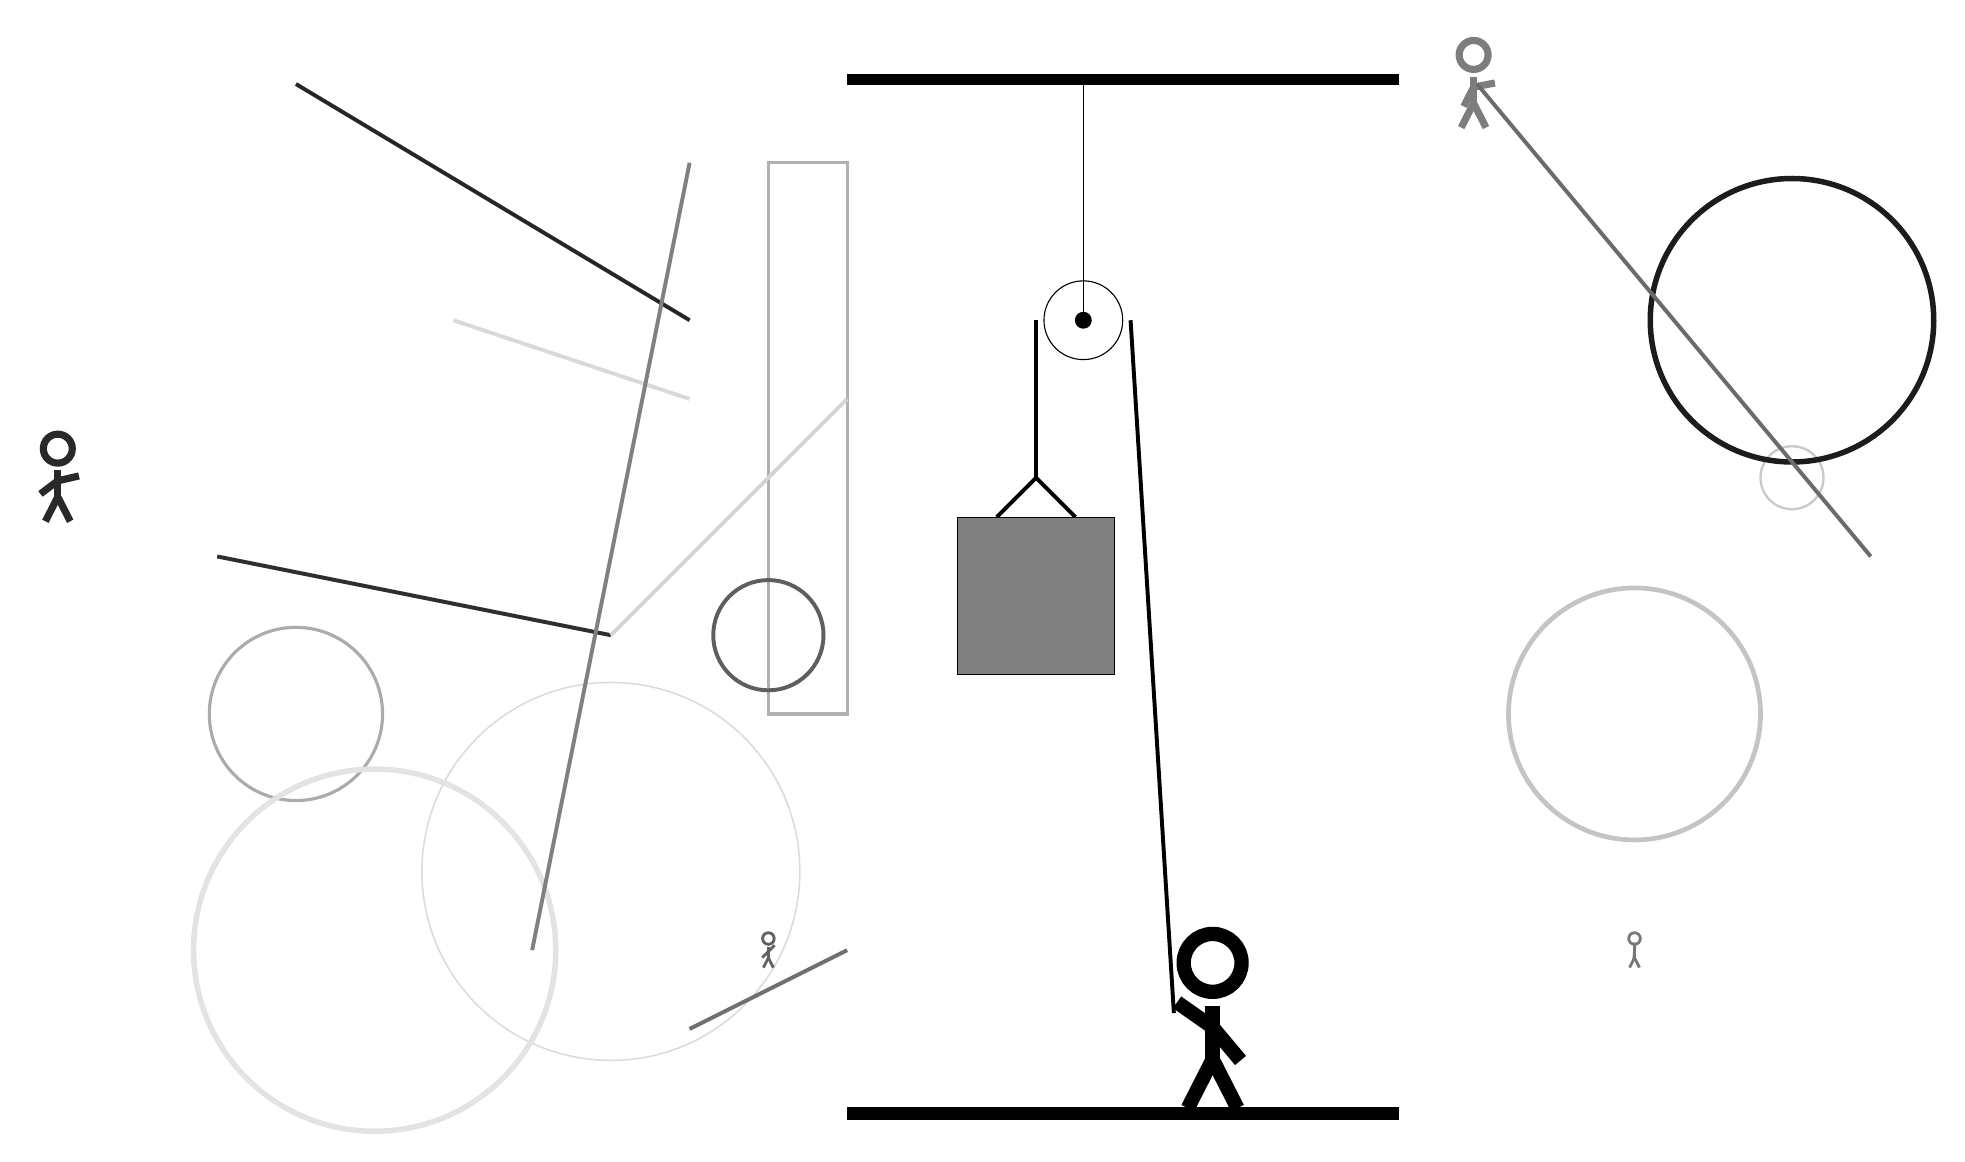
\begin{tikzpicture}
		%%%%% START %%%%%
		
		\draw[fill=black] (-2, 10) rectangle (5, 10.125);
		
		\draw (1, 7) circle (0.5);
		\draw[fill=black] (1, 7) circle (0.1);
		\draw (1, 10) -- (1, 7);
		
		\draw[line width=0.5mm, color=black!82](-5, 3) -- (-10, 4);
		
		\draw[line width=0.4mm, color=black!31] (-3, 2) rectangle (-2, 9);
		\draw[line width=0.5mm, color=black!15](-7, 7) -- (-4, 6);
		\draw [line width=0.5mm, color=black!63](-3, 3) circle (0.7);
		
		\draw [line width=0.3mm, color=black!21](10, 5) circle (0.4);
		
		\draw [line width=0.4mm, color=black!33](-9, 2) circle (1.1);
		
		\draw[line width=0.5mm, color=black!85](-4, 7) -- (-9, 10);
		\draw[line width=0.5mm, color=black!17](-5, 3) -- (-2, 6);
		\draw [line width=0.2mm, color=black!14](-5, 0) circle (2.4);
		\draw[line width=0.5mm, color=black!52](8, 0) -- (8, 0);
		\node[line width=0.4mm, color=black!62] at (-3, -1) {\Strichmaxerl[2][45][45]};
		
		\draw [line width=0.7mm, color=black!11](-8, -1) circle (2.3);
		\draw [line width=0.6mm, color=black!23](8, 2) circle (1.6);
		
		\node[line width=0.4mm, color=black!53] at (8, -1) {\Strichmaxerl[2][85][89]};
		\draw [line width=0.7mm, color=black!89](10, 7) circle (1.8);
		\node[line width=0.4mm, color=black!51] at (6, 10) {\Strichmaxerl[5][63][11]};
		
		\draw[line width=0.5mm, color=black!58](6, 10) -- (11, 4);
		\draw[line width=0.5mm, color=black!50](-4, 9) -- (-6, -1);
		\node[line width=0.4mm, color=black!84] at (-12, 5) {\Strichmaxerl[5][37][13]};
		
		\draw[line width=0.5mm, color=black!56](-2, -1) -- (-4, -2);
		
		\draw[line width=0.5mm] (-0.1, 4.5) -- (0.4, 5.0) -- (0.9, 4.5);
		\draw[fill=black!50] (-0.6, 4.5) rectangle (1.4, 2.5);
		
		\draw[line width=0.5mm] (0.4, 7) -- (0.4, 5.0);
		\centerarc[line width=0.5mm](1, 7)(0:180:0.6);
		\draw[line width=0.5mm](1.6, 7) -- (2.15, -1.8);
		
		\node at (2.6, -1.9) {\Strichmaxerl[10][-35][-50]};
		
		\draw[fill=black] (-2, -3) rectangle (5, -3.15);
		
		%%%%% END %%%%%
	\end{tikzpicture}
\end{document}